\documentclass{oci}
\usepackage[utf8]{inputenc}
\usepackage{lipsum}
\usepackage{tikz}

\title{Cubos de papel}

\begin{document}
\begin{problemDescription}

  El pequeño Nelman es un niño con mucha imaginación.
  Nunca le faltan ideas para entretener sus tardes.
  Uno de sus pasatiempos favoritos es amar cubos de papel. 
  Para armar un cubo debe primero recortar una plantilla como la que se muestra más abajo.
  Una vez cortada, puede doblarla y pegarla para armar un cubo.

\begin{center}
	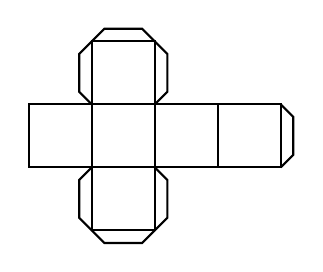
\begin{tikzpicture}[scale = 0.8]
\draw[thick] (0,0) rectangle +(1,1);
\draw[thick] (1,1) rectangle +(1,1);
\draw[thick] (1,0) rectangle +(1,1);
\draw[thick] (1,-1) rectangle +(1,1);
\draw[thick] (2,0) rectangle +(1,1);
\draw[thick] (3,0) rectangle +(1,1);
\draw[thick] (2,-1) -- (2.2,-0.8) -- (2.2,-0.2)-- (2,0);
\draw[thick] (1,-1) -- (1.2,-1.2) -- (1.8,-1.2)-- (2,-1);
\draw[thick] (1,-1) -- (0.8,-0.8) -- (0.8,-0.2)-- (1,0);
\begin{scope}[shift ={(0,2)}]
\draw[thick] (1,-1) -- (0.8,-0.8) -- (0.8,-0.2)-- (1,0);
\end{scope}
\begin{scope}[shift ={(1,1)}]
\draw[thick] (0,1) -- (0.2,1.2) -- (0.8,1.2)-- (1,1);
\end{scope}
\begin{scope}[shift ={(0,2)}]
\draw[thick] (2,-1) -- (2.2,-0.8) -- (2.2,-0.2)-- (2,0);
\end{scope}
\begin{scope}[shift ={(2,1)}]
\draw[thick] (2,-1) -- (2.2,-0.8) -- (2.2,-0.2)-- (2,0);
\end{scope}
% \begin{scope}[shift ={(0.5,0.5)}]
% \draw[fill = black] (1,1) circle (0.1);
% \draw[fill = black] (1-0.2,-1-0.2) circle (0.1);
% \draw[fill = black] (1+0.2,-1+0.2) circle (0.1);

% \draw[fill = black] (0.2,+0.2) circle (0.1);
% \draw[fill = black] (0,0) circle (0.1);
% \draw[fill = black] (-0.2,-0.2) circle (0.1);

% \draw[fill = black] (1.2,0.2) circle (0.1);
% \draw[fill = black] (0.8,0.2) circle (0.1);
% \draw[fill = black] (1.2,-0.2) circle (0.1);
% \draw[fill = black] (0.8,-0.2) circle (0.1);

% \draw[fill = black] (2,0) circle (0.1);
% \draw[fill = black] (2.2,0.2) circle (0.1);
% \draw[fill = black] (1.8,0.2) circle (0.1);
% \draw[fill = black] (2.2,-0.2) circle (0.1);
% \draw[fill = black] (1.8,-0.2) circle (0.1);

% \draw[fill = black] (3,0.2) circle (0.1);
% \draw[fill = black] (3,-0.2) circle (0.1);
% \draw[fill = black] (3.2,0.2) circle (0.1);
% \draw[fill = black] (2.8,0.2) circle (0.1);
% \draw[fill = black] (3.2,-0.2) circle (0.1);
% \draw[fill = black] (2.8,-0.2) circle (0.1);
% \end{scope}

%%El cubito

% \begin{scope}[scale={1.5}, shift={(-1.5,-0.2)}]
%   \draw[thick] (6,0) rectangle +(1,1);
%   \begin{scope}[cm={1,0,0,1,(6.5,0.5)}]
%   \draw[thick] (-0.5,-0.5) rectangle +(1,1);
%   \draw[fill = black] (0,0) circle (0.1);
%   \draw[fill = black] (0.2,0.2) circle (0.1);
%   \draw[fill = black] (-0.2,0.2) circle (0.1);
%   \draw[fill = black] (0.2,-0.2) circle (0.1);
%   \draw[fill = black] (-0.2,-0.2) circle (0.1);
%   \end{scope}

%   \begin{scope}[cm={0.5,0.5,0,1,(7,0)}]
%     \draw[thick] (0,0) rectangle +(1,1);
%     \begin{scope}[shift ={(-2.5,0.5)}]
%     \draw[fill = black] (3,0.2) circle (0.1);
%     \draw[fill = black] (3,-0.2) circle (0.1);
%     \draw[fill = black] (3.2,0.2) circle (0.1);
%     \draw[fill = black] (2.8,0.2) circle (0.1);
%     \draw[fill = black] (3.2,-0.2) circle (0.1);
%     \draw[fill = black] (2.8,-0.2) circle (0.1);
%     \end{scope}
%   \end{scope}
%   \begin{scope}[cm={1,0,0.5,0.5,(6,1)}]
%   \draw[thick] (0,0) rectangle +(1,1);
%   \draw[fill = black] (0.5,0.5) circle (0.1);
%   \end{scope}
% \end{scope}
\end{tikzpicture}
\end{center}

Recientemente, Nelman se ha dado cuenta que armar cubos es mucho más entretenido si pinta sus caras
de colores.
Nelman posee 6 colores distintos y por simplicidad siempre pinta la plantilla antes de armar el cubo
con ella.

Luego de colorear y armar cubos por muchas horas, Nelman se ha dado cuenta de algo interesante.
Algunas veces distintas formas de colorear la plantilla dan como resultado el mismo cubo.
Por ejemplo, a continuación se muestran dos formas distintas de colorear una plantilla, pero los cubos
armados a partir de estas son indistinguibles (este corresponde al primer caso de ejemplo mostrado
al final del enunciado).

	\begin{center}
	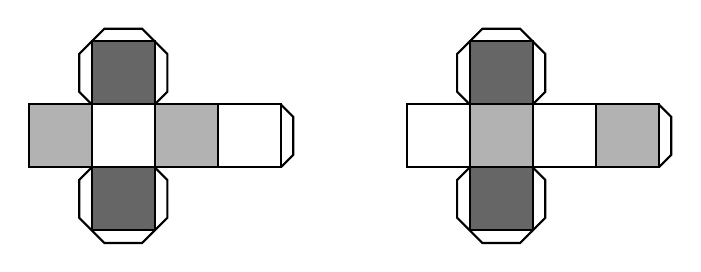
\begin{tikzpicture}[scale = 0.8]
	\draw[thick, fill=black!30] (0,0) rectangle +(1,1);
	\draw[thick, fill=black!60] (1,1) rectangle +(1,1);
	\draw[thick] (1,0) rectangle +(1,1);
	\draw[thick, fill=black!60] (1,-1) rectangle +(1,1);
	\draw[thick, fill=black!30] (2,0) rectangle +(1,1);
	\draw[thick] (3,0) rectangle +(1,1);
	\draw[thick] (2,-1) -- (2.2,-0.8) -- (2.2,-0.2)-- (2,0);
	\draw[thick] (1,-1) -- (1.2,-1.2) -- (1.8,-1.2)-- (2,-1);
	\draw[thick] (1,-1) -- (0.8,-0.8) -- (0.8,-0.2)-- (1,0);
	\begin{scope}[shift ={(0,2)}]
	\draw[thick] (1,-1) -- (0.8,-0.8) -- (0.8,-0.2)-- (1,0);
	\end{scope}
	\begin{scope}[shift ={(1,1)}]
	\draw[thick] (0,1) -- (0.2,1.2) -- (0.8,1.2)-- (1,1);
	\end{scope}
	\begin{scope}[shift ={(0,2)}]
	\draw[thick] (2,-1) -- (2.2,-0.8) -- (2.2,-0.2)-- (2,0);
	\end{scope}
	\begin{scope}[shift ={(2,1)}]
	\draw[thick] (2,-1) -- (2.2,-0.8) -- (2.2,-0.2)-- (2,0);
	\end{scope}
	
	\begin{scope}[shift ={(6,0)}]
	\draw[thick] (0,0) rectangle +(1,1);
	\draw[thick, fill=black!60] (1,1) rectangle +(1,1);
	\draw[thick, fill=black!30] (1,0) rectangle +(1,1);
	\draw[thick, fill=black!60] (1,-1) rectangle +(1,1);
	\draw[thick] (2,0) rectangle +(1,1);
	\draw[thick, fill=black!30] (3,0) rectangle +(1,1);
	\draw[thick] (2,-1) -- (2.2,-0.8) -- (2.2,-0.2)-- (2,0);
	\draw[thick] (1,-1) -- (1.2,-1.2) -- (1.8,-1.2)-- (2,-1);
	\draw[thick] (1,-1) -- (0.8,-0.8) -- (0.8,-0.2)-- (1,0);
	\begin{scope}[shift ={(0,2)}]
	\draw[thick] (1,-1) -- (0.8,-0.8) -- (0.8,-0.2)-- (1,0);
	\end{scope}
	\begin{scope}[shift ={(1,1)}]
	\draw[thick] (0,1) -- (0.2,1.2) -- (0.8,1.2)-- (1,1);
	\end{scope}
	\begin{scope}[shift ={(0,2)}]
	\draw[thick] (2,-1) -- (2.2,-0.8) -- (2.2,-0.2)-- (2,0);
	\end{scope}
	\begin{scope}[shift ={(2,1)}]
	\draw[thick] (2,-1) -- (2.2,-0.8) -- (2.2,-0.2)-- (2,0);
	\end{scope}
	\end{scope}
	
	\end{tikzpicture}
	\end{center}
	
De manera formal, diremos que dos cubos son iguales si existe alguna forma de rotarlos de modo
que se vean idénticos.
A Nelman le gustaría saber si dadas dos formas de colorear una plantilla estas dan como resultado el
mismo cubo.
De esta forma no gastará tiempo innecesario armando cubos iguales.
?`Podrías ayudarlo?
% Puedes ayudar al pequeño Nelman a decidir si dos formas de colorear un  producen el mismo cubito?

\end{problemDescription}

\begin{inputDescription}
  La entrada consiste en dos líneas.
  Cada una describe una forma de colorear una plantilla usando $6$ números enteros $a_1$ $a_2$
  $a_3$ $a_4$ $a_5$ $a_6$ todos entre $0$ y $5$.
  Estos números representan el color para cada una de las seis caras del cubo en el orden que se
  muestra en la siguiente imagen.

\begin{center}
	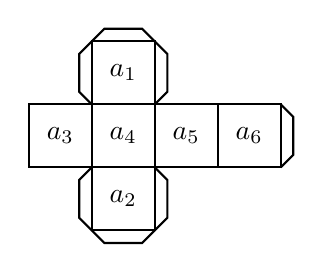
\begin{tikzpicture}[scale = 0.8]
	\draw[thick] (0,0) rectangle +(1,1);
	\draw[thick] (1,1) rectangle +(1,1);
	\draw[thick] (1,0) rectangle +(1,1);
	\draw[thick] (1,-1) rectangle +(1,1);
	\draw[thick] (2,0) rectangle +(1,1);
	\draw[thick] (3,0) rectangle +(1,1);
	\draw[thick] (2,-1) -- (2.2,-0.8) -- (2.2,-0.2)-- (2,0);
	\draw[thick] (1,-1) -- (1.2,-1.2) -- (1.8,-1.2)-- (2,-1);
	\draw[thick] (1,-1) -- (0.8,-0.8) -- (0.8,-0.2)-- (1,0);
	\begin{scope}[shift ={(0,2)}]
	\draw[thick] (1,-1) -- (0.8,-0.8) -- (0.8,-0.2)-- (1,0);
	\end{scope}
	\begin{scope}[shift ={(1,1)}]
	\draw[thick] (0,1) -- (0.2,1.2) -- (0.8,1.2)-- (1,1);
	\end{scope}
	\begin{scope}[shift ={(0,2)}]
	\draw[thick] (2,-1) -- (2.2,-0.8) -- (2.2,-0.2)-- (2,0);
	\end{scope}
	\begin{scope}[shift ={(2,1)}]
	\draw[thick] (2,-1) -- (2.2,-0.8) -- (2.2,-0.2)-- (2,0);
	\end{scope}
	\begin{scope}[shift ={(0.5,0.5)}]
	\node at (0,0) {$a_3$};
	\node at (1,0) {$a_4$};
	\node at (2,0) {$a_5$};
	\node at (3,0) {$a_6$};
	\node at (1,1) {$a_1$};
	\node at (1,-1) {$a_2$};
	\end{scope}
	\end{tikzpicture}
\end{center}
\end{inputDescription}

\begin{outputDescription}
  Si las dos formas de colorear las plantillas dan como resultado el mismo cubo la salida debe
  contener un $1$.
  En caso contrario debe contener un $0$.
\end{outputDescription}

\begin{scoreDescription}
  Este problema no contiene subtareas.
  Se evaluarán exactamente 200 casos de prueba y se otorgará puntaje de acuerdo a la cantidad de
  casos correctos.
  Si $C$ es la cantidad de casos correctos, el puntaje recibido será $\max(C-100,0)$. 
\end{scoreDescription}

\begin{sampleDescription}
\sampleIO[0.5][0.5]{sample-1}
\vspace{-1em}
    Este es el ejemplo descrito en el enunciado.
    Las caras de color gris oscuro están descritas con un 1, las de gris claro con un 2 y las en
    blanco con un 3.
\vspace{1em}

\sampleIO[0.5][0.5]{sample-2}
\sampleIO[0.5][0.5]{sample-3}
\end{sampleDescription}

\end{document}
